\documentclass[a4paper,12pt]{article}
\setlength{\headheight}{68.803pt}
\addtolength{\topmargin}{-56.803pt}

\usepackage[utf8]{inputenc}
\usepackage[T1]{fontenc}
\usepackage{lmodern}
\usepackage[nopatch=footnote]{microtype}
\usepackage{fvextra}
\DefineVerbatimEnvironment{Verbatim}{Verbatim}{
  breaklines=true,
  breakanywhere=true,
  frame=single,
  fontsize=\small
}

\usepackage[
  left=1in,
  right=1in,
  top=3cm,
  bottom=1in
]{geometry}

\usepackage[
    colorlinks=true,
    linkcolor=black,
    urlcolor=blue,
    citecolor=blue,
    pdfborder={0 0 0},
    pdfauthor={Massimo Mantineo},
    pdftitle={Meccanismi di Sincronizzazione},
    pdfsubject={Laboratorio di Reti e Sistemi Distribuiti: HANDS-ON 11},
]{hyperref}

\usepackage{graphicx}
\graphicspath{{../../assets/}{../../assets/ho1/}{../../assets/ho2/}{../../assets/ho3/}{../../assets/ho4/}{../../assets/ho5/}{../../assets/ho6/}{../../assets/ho7/}{../../assets/ho8/}{../../assets/ho10/}}
\usepackage{tikz}
\usetikzlibrary{positioning, arrows.meta, shapes.symbols}
\usepackage{listings}
\usepackage{xcolor}
\usepackage{amsmath, amssymb}
\usepackage{fancyhdr}
\usepackage{setspace}
\usepackage{pgfplots}
\pgfplotsset{compat=1.17}
\usepackage{booktabs}
\usepackage[skins, listings]{tcolorbox}
\usepackage{float}

\newtcblisting{terminal}[1][]{
    listing only,
    colback=black!85!white,
    colframe=black!70!white,
    colupper=green!80!white,
    coltitle=white,
    title=#1,
    fonttitle=\bfseries\sffamily,
    listing options={
        language={},
        basicstyle=\ttfamily\small\color{green!80!white},
        backgroundcolor={},
        frame=none,
        breaklines=true,
        showstringspaces=false,
        numbers=none
    },
    enhanced,
    drop shadow,
    arc=3mm
}

\newtcblisting{ccode}[1][]{
    listing only,
    colback=blue!3!white,
    colframe=blue!70!black,
    title=#1,
    fonttitle=\bfseries\sffamily,
    listing options={
        style=cstyle,
        backgroundcolor={},
        frame=none
    },
    enhanced,
    drop shadow,
    arc=3mm
}

\setlength{\footskip}{50pt}

\lstdefinestyle{cstyle}{
    language=C,
    basicstyle=\ttfamily\small,
    numbers=left,
    numberstyle=\tiny,
    stepnumber=1,
    numbersep=5pt,
    backgroundcolor=\color{white},
    showspaces=false,
    showstringspaces=false,
    showtabs=false,
    frame=single,
    tabsize=4,
    captionpos=b,
    breaklines=true,
    breakatwhitespace=true,
    keywordstyle=\color{blue}\bfseries,
    commentstyle=\color{green!50!black},
    stringstyle=\color{red},
}
\lstset{style=cstyle}

\pagestyle{fancy}
\fancyhf{}

\fancyhead[L]{%
  \parbox[b]{0.45\textwidth}{%
    \small
    Student Name: Massimo Mantineo\\
    Student ID: 541924
    \vspace{20pt}
  }%
}
\fancyhead[C]{%
  \parbox[b]{0.2\textwidth}{%
    \centering
    \normalsize \bfseries
    LabReSiD25\\
    Hands-On 11
    \vspace{20pt}
  }%
}
\fancyhead[R]{%
  \parbox[b]{0.35\textwidth}{%
    \flushright
    \includegraphics[width=3.5cm]{\detokenize{logo_unime_orizontale.png}}
    \vspace{15pt}
  }%
}

\renewcommand{\contentsname}{Indice}

\title{\vspace{-2cm}Report: Meccanismi di Sincronizzazione\\
\large (Hands-On 11)}
\author{Massimo Mantineo \\ Matricola: 541924}
\date{MESSINA, A.A. 2024/2025}

\begin{document}

\begin{titlepage}
    \thispagestyle{empty}
    \centering
    \vspace*{1cm}
    \includegraphics[width=6cm]{\detokenize{logo_unime_orizontale.png}}\par\vspace{1cm}
    \vspace{2cm}
    {\Large \textbf{Università degli Studi di Messina}\par}
    {\large Dipartimento MIFT - Corso di Laurea Triennale in Informatica (L-31)\par}
    \vspace*{1cm}
    {\large Laboratorio di Reti e Sistemi Distribuiti\par}
    \vspace{1cm}
    {\Large \textbf{HANDS-ON 11:}\\
    Meccanismi di Sincronizzazione tra Thread\par}
    \vspace{2cm}
    {\large Massimo Mantineo \par}
    {\large Matricola: 541924 \par}
    \vfill
    {\large Messina, A.A. 2024/2025 \par}
\end{titlepage}

\clearpage
\pagestyle{fancy}
\tableofcontents
\newpage

\section{Problem Statement}
L'undicesima esercitazione (HO11) è focalizzata sulle problematiche della concorrenza nei paradigmi di programmazione multithreading, in particolar modo sull'individuazione e risoluzione delle *Race Conditions*. 
L'obiettivo si articola in tre task principali: 
1. La realizzazione di un programma in cui 10 thread incrementano un contatore globale condiviso all'interno di una *sezione critica*, senza tuttavia avvalersi di meccanismi di sincronizzazione. 
2. La risoluzione della medesima operazione ricorrendo a costrutti per la Mutua Esclusione (*Mutex*).
3. L'implementazione di un differente scenario in cui l'accesso alla sezione critica da parte di 5 thread viene limitato per permettere l'ingresso massimo a due soli thread alla volta, sfruttando l'astrazione concettuale dei Semofori posix a conteggio limitato.

\section{Stato dell'Arte}
Le problematiche sollevate nell'Hands-On 11 costituiscono le fondamenta della programmazione concorrente:
\begin{itemize}
    \item \textbf{Sezione Critica e Condizioni di Corsa}: Si verifica quando più flussi di esecuzione (es. thread) accedono simultaneamente e in modalità non atomica a informazioni condivise (memoria, variabili). La mancanza di atomicità espone le operazioni d'aggiornamento a sovrascritture incrociate al momento della schedulazione del sistema operativo.
    \item \textbf{Mutex (Mutual Exclusion)}: Costituisce il costrutto nativo delle specifiche \texttt{Pthreads} (tramite \texttt{pthread\_mutex\_t}) per implementare il blocco (\textit{lock}) granulare all'ingresso della sezione critica e lo sblocco (\textit{unlock}) all'uscita. Garantisce formalmente che solo un thread possa trovarsi all'interno del proprio perimetro in ogni dato istante temporale.
    \item \textbf{Semofori (Counting Semaphores)}: Strumento di generalizzazione (gestito via \texttt{<semaphore.h>}). A differenza di un mutex (che è assimilabile spesso a un semaforo binario controllante una sola risorsa esatta), un semaforo inizializzato a $N$ protegge l'accesso limitato ad $N$ entità. I thread usano \texttt{wait()} per acquisire un token, causandone decremento, e \texttt{post()} per rilasciarlo al termine dell'operazione.
\end{itemize}

\section{Metodologia ed Implementazione}
Per coprire gli obiettivi prestabiliti, l'ecosistema del laboratorio fa uso della libreria \texttt{<pthread.h>} nello standerd POSIX e \texttt{<semaphore.h>} per le varianti col semaforo.

\begin{figure}[H]
    \centering
    \begin{tikzpicture}[
        node distance=1cm and 2cm,
        thread/.style={circle, draw=blue!70, fill=blue!5, thick, minimum size=1cm, font=\tiny\bfseries},
        resource/.style={rectangle, draw=green!70, fill=green!5, thick, minimum width=1.5cm, minimum height=1cm, font=\tiny\bfseries},
        lock/.style={draw=red!70, fill=red!5, thick, shape=rectangle, rounded corners, minimum width=1.2cm, font=\tiny\itshape},
        arrow/.style={-Stealth, thick, gray!80}
    ]
        % Mutex Side
        \node[resource] (res1) {Shared Resource};
        \node[lock, above=0.3cm of res1] (mutex) {Mutex Lock};
        \node[thread, left=of mutex] (t1) {Thread A};
        \node[thread, below=0.5cm of t1] (t2) {Thread B};
        
        \draw[arrow] (t1) -- node[above, font=\tiny] {Lock} (mutex);
        \draw[arrow, dashed] (t2) -- node[below, font=\tiny] {Waiting} (mutex);
        
        % Semaphore Side
        \node[resource, right=5cm of res1] (res_pool) {Resource Pool (N=2)};
        \node[lock, above=0.3cm of res_pool] (sem) {Semaphore (Count=1)};
        \node[thread, left=1cm of sem] (t3) {Thread C};
        \node[thread, below=0.5cm of t3] (t4) {Thread D};
        \node[thread, below=0.5cm of t4] (t5) {Thread E};
        
        \draw[arrow] (t3) -- node[above, font=\tiny] {Wait} (sem);
        \draw[arrow] (t4) -- node[below, font=\tiny] {Wait} (sem);
        \draw[arrow, dashed] (t5) -- node[below, font=\tiny] {Blocked} (sem);

        % Labels
        \node[above=0.8cm of mutex, font=\bfseries\small] {MUTUAL EXCLUSION};
        \node[above=0.8cm of sem, font=\bfseries\small] {COUNTING SEMAPHORE};
    \end{tikzpicture}
    \caption{Differenza concettuale tra Mutex (Esecuzione Esclusiva) e Semaforo (Accesso Limitato a pool).}
    \label{fig:sync\_mechanisms}
\end{figure}

\subsection{Race Condition Senza Sincronizzazione}
Nel primissimo passo viene volutamente violata la sincronizzazione. Il \texttt{shared\_counter++} viene eseguito da 10 thread 10.000 volte ciascuno.
\begin{ccode}[Snippet Esercizio 1: Assenza di controllo in Sezione Critica]
void* thread\_function(void* arg) {
    long thread\_id = (long)arg;
    for (int i = 0; i < MAX\_VALUE; i++) {
        shared\_counter++; // <--- Non atomico: Read, Increment, Write
    }
    printf("Thread %ld: shared\_counter = %d\n", thread\_id, shared\_counter);
    pthread\_exit(NULL);
}
\end{ccode}

\subsection{Mutua Esclusione con Mutex}
L'approccio corretto del medesimo codice precedente fa uso del lock della libreria pthread passandogli l'indirizzo di un \texttt{counter\_mutex}.
\begin{ccode}[Snippet Esercizio 2: Controllo tramite Mutex]
for (int i = 0; i < MAX\_VALUE; i++) {
    pthread\_mutex\_lock(&counter\_mutex);
    shared\_counter++; // <--- Protetto al 100% da accesso multi-thread
    pthread\_mutex\_unlock(&counter\_mutex);
}
\end{ccode}

\subsection{Gestione della Concorrenza Parziale (Semofori)}
Il terzo esercizio introduce l'entità \texttt{sem\_t} di cui si decreta in fase di inizializzazione un contatore esatto di concorrenza.
\begin{ccode}[Snippet Esercizio 3: Semaforo max limit 2]
sem\_wait(&max\_concurrency\_sem); // Thread attende il token
// ... Critical Section accessibile per due thread contemporanei ...
sleep(2); // Lavoro pesante simulato
sem\_post(&max\_concurrency\_sem); // Ritiro e rilascio
\end{ccode}
Il cui setup del semaforo poggia sulla chiamata \texttt{sem\_init(\&max\_concurrency\_sem, 0, 2);}.


\subsection{Istruzioni di Esecuzione}
L'applicativo viene gestito interamente tramite Makefile:
\begin{terminal}[Build & Run]
$ make
$ ./programma
\end{terminal}

\section{Risultati}
L'esecuzione della pipeline ha restituito un comportamento pienamente conforme all'osservazione teorica.

\subsection{Output Senza Sincronizzazione}
\begin{terminal}[Output di esecuzione ex1\_no\_sync]
massimo@PORTATILE-Linux:~/Scrivania/LabReSid24-25/hands-on/ho11$ ./ex1\_no\_sync
Thread 9: shared\_counter = 76935
Final value of shared\_counter: 76935 (Expected: 100000)
\end{terminal}
La chiara denotazione di "informazione perduta" riflette statisticamente che le operazioni non sono avvenute correttamente.

\subsection{Output con Sincronizzazione Mutex}
\begin{terminal}[Output di esecuzione ex2\_sync]
massimo@PORTATILE-Linux:~/Scrivania/LabReSid24-25/hands-on/ho11$ ./ex2\_sync
Thread 4: shared\_counter = 100000
Final value of shared\_counter: 100000 (Expected: 100000)
\end{terminal}
Con un perimetro sincronizzato l'incremento di ogni esecuzione finisce esattamente alla cifra teoricamente attesa di 100.000 (10.000 incremento a thread $\times$ 10 thread allocati).

\subsection{Output Multi-Accesso Semaforo}
\begin{terminal}[Output di esecuzione ex3\_semaphore]
massimo@PORTATILE-Linux:~/Scrivania/LabReSid24-25/hands-on/ho11$ ./ex3\_semaphore
Thread 0 has ENTERED the critical section.
Thread 1 has ENTERED the critical section.
Thread 2 is waiting to enter the critical section...
Thread 4 is waiting to enter the critical section...
Thread 3 is waiting to enter the critical section...
Thread 0 is LEAVING the critical section.
Thread 1 is LEAVING the critical section.
Thread 2 has ENTERED the critical section.
\end{terminal}
Solo all'uscita delle coppie 0-1 scatta lo sblocco in grado di far defluire il Thread 2 rimasto bloccato in attesa sul Semaforo.

\section{Conclusioni e Sviluppi Futuri}
L'Hands-On 11 offre la prova empirica definitiva che lo scambio di memoria in ambito multithreading non può mai assumere la connotazione dell'idempotenza se non attraverso un sistema regolamentato di Mutex, Monitor o Semafori. Si è osservato come l'implementazione pratica del Mutex garantisca sicurezza, sacrificando inevitabilmente il parallelismo perfetto nel punto interessato.

\noindent \textbf{Sviluppi futuri:}
\begin{itemize}
    \item \textbf{Deadlock Prevention}: Esplorare l'implementazione di sistemi di priorità e ordine logico formale nell'acquisizione di mutex multipli paralleli ai fine da evitare che due thread si blocchino permanentemente su lock ciclici (Deadlocks).
    \item \textbf{Rwlocks (Read-Write Locks)}: Implementare soluzioni avanzate che consentano l'accesso parallelo e contemporaneo alla lettura dei dati ma rendano vincolante la mutua esclusione solo per la scrittura, ottimizzando fortemente contesti ove è richiesta un'informazione aggiornata ma raramente modificata.
\end{itemize}

\end{document}
